%%% -*-LaTeX-*-

\chapter{The Multi-cluster Trading Mechanism}

As the adoption of multi-cluster environments accelerates and the
infrastructure continues to evolve to support more use-cases, we are presented
with an opportunity to build tools on top of that and leverage the existing
networking innovations to optimize how clusters interact in a multi-cluster
environment. Since a multi-cluster environment is a loose definition, we define
our multi-cluster environment as a one which clusters are discoverable to one
another and implements the trading mechanism's API.

We argue that it is possible to increase cluster resource utilization,
decrease average job completion time, and/or reduce average cost by providing
clusters with a resource trading mechanism allowing the virtual sharing of
resources across clusters. 

The trader is the component putting the mechanism in effect. It involves
receiving policies as input from the user, communicating with other clusters'
traders and facilitating the exchange of resources between them. It is the
point of contact between the foreign clusters and the host cluster's scheduler.

In this chapter we present the system design, discuss the role of the scheduler
in the mechanism, explain what user-defined policies are and lastly describe
the design of the trader itself. 

\begin{figure}[H]
  \centerline{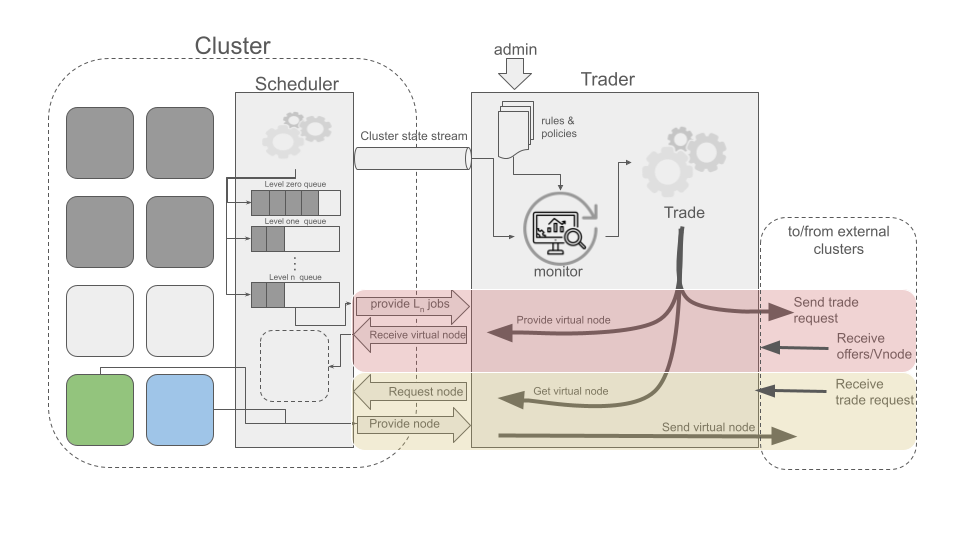
\includegraphics[scale=0.45]{figures/system-diagram}}
  \caption{System architecture showing the various compononents of the trader,
    and how it connects to a cluster. Red section represents the procedure
    requesting resources and the yellow section depicts the procedure of
    providing resources to external clusters. squares represents the node in
    the host cluster. Dark gray nodes represent localy utilized nodes and light
    gray nodes represent free local nodes. Green and blue nodes represent
    resources    provided to external clusters and the dotted square is a
    virtual node received from an external cluster} 
  \figlabel{fig1}
\end{figure}

\section{Scheduler}
% introducing the notion of minimal intursivity
\subsection{Requirements}
Cluster scheduling have been widely studied and remains a prominent area of
research. Our objective in relation to scheduling is not to replace the
clusters' scheduling algorithm nor interfere with its scheduling decisions, but
to improve the cluster's performance while minimizing friction and interaction
with the trader. It it also worth noting that the scheduler does not directly
interact with the broader multi-cluster environment but only with its own
trader, reducing the communication surface area and keeping local scheduling
independent from the mechanism. [NEEDS BETTER WORDING]

The scheduler's role in the mechanism comprises of passing on cluster state to
local trader, providing resources for trades, and receiving resources from
trades. Cluster state are measurements necessary to inform trading decisions.
These metrics are typically collected in cluster schedulers for performance
analysis and monitoring and include wait time, cost of compute/memory,
utilization etc.

\noindent Providing and receiving resources are an extension of the cluster's
ability to add new nodes and allocate resources on existing ones. 

Thus scheduling is detached from trading and only an interface is required to
connect the two modules together, allowing any scheduling algorithm already
running in a cluster to remain unchanged. This lays the ground to the general
requirements for a scheduler to operate in the mechanism, and shows that a
specific scheduling algorithm is not required for our mechanism. With that
being said, we now present our scheduling algorithm and discuss the underlying
design decisions. 

\subsection{Design}
% delay scheduling 

The base of our scheduling algorithm is delay scheduling [CITE] due to its
simplicity and []focus on data locality. In delay scheduling, a job is first
assigned the lowest level 0, allowing it to only be scheduled on the node its
data is at. The job is subsequently bumbed to higher levels as it fails to get
it scheduled in close proximity, permitting the scheduler to schedule the job
further away from its data as the wait time of the job increases. Consequently
the leveling represent the job's expectated distance from its data. This notion
of proximity and gradual drifting[] is extended to include external clusters in
our mechanism. Jobs already anticipating poor data locality would be the ones
more likely to be scheduled on an external cluster. This insures fair
scheduling even as we extend the scope of scheduling to a multi-cluster
environment. These jobs would also incur the least percentage reduction in
performance when scheduled in a foreign cluster.

\figref{fig1} includes the architecture of the scheduler described here. The
different queues represent different levels a job can be in. The incoming and
outgoing arrows represents the exposed interface the trader utilize to
communicate with the scheduler and will be further explained next.

%Of course, more analysis could go in deciding what jobs would better fit being
%exported to other clusters like jobs demanding less communiication with other
%jobs in the cluster, jobs with less data dependency, ..., but this is out of
%scope of this thesis.


% research idea: data locality-aware scheduling research is trying to get the
% jobs scheduled next to data, no study i encountered actually socres the
% sensitivity of the jobs in relation to other jobs in the cluster. (probably
% for fairness concerns) but might be an interesting project to work on. 

%This presents us with a clean heuristic when calculalting resources needed for
%trading. As the level of the of what to include in our 


\section{Trader} \label{trader}

The trader is the central component of the mechanism. It facilitates the
exchange of resources between clusters and encapsulates all trading logic. 

This exchange is bidirectional, meaning a cluster can receive external
resources and give away its own resources to other clusters. Clusters only
communicate with each other through their traders, which gets configured by the
cluster adminstrator. 

%Incentive intro
Traders can either be cooperative or opportunistic. In a cooperative trading
environment, trading does not need an incentive, and furthers the overall
performance of the participating clusters. A straightforward use-case to this
model is organizations with multiple clusters; allowing the exchange of
resources benefits the organization as a whole. The opportunistic model
facilitates trading between self-serving clusters by introducing a monetary
incentive in a trade. Traders would way in the cost and profit of participating
in a trade and that would be the primary motivation to giveaway resources.  

The trader is responsible for keeping the cluster's state in conformity with a
desired state. As shown in the figure, the trader establishes a cluster state
stream with the scheduler, continously receiving up-to-date cluster
information. This information includes the overall cluster utilization, average
job completion time, and current cost of resources. This stream allows the
trader to monitor and make trading decisions based on the current state of the
cluster. The desired state is declared through a set of rules, which are
configurations dynamically passed to the trader shown below:  

\begin{figure}[H]
  \begin{lstlisting}[language=go]
    type Rule struct {
      Condition: // desired state to maintain
      Action: // algorithm to use
      Broken(cluster state, condition) bool
    } 
  \end{lstlisting}
  \caption{Rules}
\end{figure}

The rule's condition represents the desired state of a measurement sent by the
scheduler to the trader, like utilization below 80\%. The rule implements a
Broken method which allows the trader to run an action when the actual cluster
state differs from the desired state. As the trader continously monitors the
cluster state, it runs the broken methods of all rules to check whether any is
broken.

The following algorithm details what happens when a rule is broken, also marked
in red in \figref{fig1} 

\begin{figure}[H]
\begin{algorithm}[H]
\caption{Outgoing Trading Algorithm}
\begin{algorithmic}
  \Procedure{Trade}{$R_b$} \Comment{$R_b$ = broken rule}
    \State $R_{action} \gets Action(R_b)$
    \State $level_N Jobs \gets GetJobs(n)$ \Comment{get from scheduler}
    \State $virtualNodeSize \gets calculateNodeSize(R_{action}, level_N Jobs)$
    \If{Incentivized}
      \State $incentive \gets calculateIncentive()$
    \EndIf
    \For{traders in multi-cluster environment}
      \State $contract \gets SendTradeRequest(virtualNodeSize, incentive)$
    \EndFor
    \State $contracts \gets ReceiveTradeResponses$ \Comment{list of approved contracts}
    \State \textbf{return} $contract_{best}$\Comment{best virtual node is sent to scheduler}
  \EndProcedure
\end{algorithmic}
\end{algorithm}
\caption{Outgoing Trading Algorithm}
\end{figure}

When a rule is broken, the trader's first step is to estimate the resources it
needs to request from other traders. Requested resources are abstracted as a
virtual node. A virtual node includes the needed resources, time, and other
constraints like hardware or OS needed for the jobs to run. Virtual nodes 
translate to the total resources acquired in the external cluster, not into a
physical node. 

% The trader specifies the smallest partition it accepts in the
% contract, usually the size of the smallest job it has in the jobs list.

The resource estimate is calculuated by first requesting the last level jobs
from the scheduler, resembling the jobs that would already be scheduled further
away from their data. The rule's action variable specifies how to estimate the
needed resources. There are currently two ways to estimate the resource
request:

\begin{enumerate}

  \item \textbf{Efficient Stacking:} A greedy approach that stacks jobs
    efficiently over time on the requested node. Starts with oldest job in the
    $level_N$ queue and add one job at a time while minimizing the size of the
    node until all jobs are included in the estimation or a constraint is
    reached.

  \item \textbf{Zero Wait:} An approach that starts jobs in queue at the same
    time. Starts with oldest job and adds one job at a time at $t_0$ until all
    jobs are included in the estimation or a constraint is reached.

\end{enumerate}

Efficient stacking allows the trader to reduce the size of the virtual node
which in turn reduces the cost of the trade and increases the chances of it
getting approved, however at a higher computation cost. Zero wait increases the
possible benefit from a trade at a higher cost per node and lower computation
cost.  

Virtual nodes have constraints like a maximum number of cores,
size of memory, time, or a budget. 

%version more appealing on a lower budget. It would be advantagous to request
%resources from another trader if it is cheaper than scaling up the cluster
%size. [Might want to introduce budgeting a bit earlier]

After estimaing the needed resources, the trader calculates the incentive if
it's participating in an opportunistic model. Incentives are determined by the
cost of internally scaling up the cluster, if that is possible, the
severity of the broken rules, and the budget assigned for trading.

The trader then broadcasts a contract to all participating clusters, and waits
for replies. After receiving approved contracts, the trader approves either
approves the first contract it gets, or the best contract if a criterion is
passed, and then receives the virtual node information from the foreign trader.
It then sends the virtual node information for the scheduler to start
scheduling jobs on it.

There are various ways to rank contracts, like cost and physical proximity. 

The trader is also responsible for accepting or rejecting incoming requests.
This functionality is outlined in the yellow section in \figref{fig1} and
detailed in the following algorithm: 

\begin{figure}[H]
\begin{algorithm}[H]
\caption{Incoming Trading Algorithm}
\begin{algorithmic}
  \Procedure{ApproveTrade}{$contract$} \Comment{$contract$ = trade request}
    
    \If{$ ccs \leq contract.resources$} \Comment{ccs = current cluster state}
      \State \textbf{return} $false$ \Comment{couldn't approve trade}
    \EndIf

    \For{$P$ in Policies}
      \If{$P(ccs, T_{request}) \not= true$} 
      \State \textbf{return} $false$ \Comment{couldn't approve trade}
      \EndIf
    \EndFor
    \State $contract_r \gets sendTradeResponse$ \Comment{$contract_r$ = trade response}
    \State $contract_a \gets receiveContractApproval$ \Comment{$contract_a$ = approved trade}

    \State $virtualNode \gets getVirtualNode(T_{request})$ \Comment{from scheduler}    
    \State \textbf{return} virtualNode \Comment{Trade Approved}
  \EndProcedure
\end{algorithmic}
\end{algorithm}
\caption{Incoming Trading Algorithm}
\end{figure}

After receiving a trade request as a contract from other traders, the trader
first checks if there's enough resources in the cluster to accommodate the
trade, then loops over a set of trading policies set by the cluster admin.
Policies are symmetrical to rules for incoming requestes. They dictate how the
trader responds to received resource requests. The structure of a policy is
as follows:

\begin{figure}[H]
  \begin{lstlisting}[language=go]
    type Policy struct {
      Conditions // cluster state that allows approval
      Incentive // offer from external cluster
      ApproveRequest(request) bool 
    } 
  \end{lstlisting}
  \caption{Custom Policy implements an approveRequest method}
\end{figure}

Conditions are a set of variables that specify the acceptable threshold cluster
state should be in order to accept a trade. For each policy, the minimum
incentive is also specified which can be a function of the conditions,
decreasing if the cluster is not busy. Lastly, ApproveRequest() is the method
the trader run to know if it is okay to accept a trade according to this
policy.

If all policies approve the trade, the trader sends the a positive trade responseand waits for the requesting trader to approve the contract. Once the contract is approved, the trader then requests the resources to be reserved from the scheduler, creates the virtual node and sends it to the requesting trader. 

% add trading request algorithm

%The user defined outgoing policy also dictates any additional constraints the
%trader is required to adhere to. If the notion of a currency is established in
%the multi-cluster environmnet, constraints would include a budget, as well as a
%maximum price to pay for resources, which can be the price of renting out the
%resources from the vendor, or a cost estimate anaylsis algorithm. 

% rules intro
%A desired state is the state the orchestrator works on acheiving and keeping. A
%cluster adminstrator passes the desired state to the orchestrator, which in
%turn continously checks the actual state and compares it to the desired state
%while trying to restore the actual state to the desired one when it deviates.
%For example, if the desired state of a job on the cluster is having 3 replicas,
%and one server crashes, deleting one of the job's replicas, the orchestrator
%finds another healthy server to run the job's third replica on.  


%the conditions under which the the cluster begins requesting resources from
%external clusters.
% policies intro

%Both rules and policies act as knobs to tune the mechanism and update it as
%cluster state and requirements change. They are pluggable and mutable, meaning
%each cluster admin can implement their own and dynamically update them as
%cluster requirements and conditions change.
%
%The metrics in scope are the ones sent by the scheduler, and include wait time,
%job completion time, utilization, cost, etc. 
%
%We design both rules and policies as interfaces, enabling them to
%be pluggable and user-defined. Policies implement an
%\texttt{approveRequest()} method, which returns true when an external trader's
%request is feasible, where as rules implement a \texttt{Broken()} method
%signature, triggering the trader to request resources when the cluster state
%breaks the conditions.  
%
%A cluster admin aiming to reduce wait time would create a rule that breaks when
%average wait time exceeds the specified threshold, and a policy that refuses to
%provide resources under similar conditions. Optimizing for utilization, an
%admin would create a rule that breaks when utilization surpasses a resource
%utilization threshold and a policy that denies resources for the same
%criterion. Tuning the policies as requirements change can be achieved by
%increasing or decreasing the respective thresholds. Stopping all trading rules
%and policies is another way to adjust the mechanism. An admin might disable
%policies altogether during peak times to enhance system predictability. 

% TRADER SECTION START

%Our mechanism offers bidirectional trading, allowing clusters to trade
%resources with one another. It also enables trading with multiple clusters, so
%clusters can trade resources with more than one cluster at a time.
%\label{sched-overhead} The following algorithms show a simple representation
%of the system, with resource utilization as the optimized-for metric:
%\label{example}
